\documentclass[12pt]{article}
\usepackage[margin=1in]{geometry}
\usepackage{mathrsfs}
\usepackage{amsmath}
\usepackage[font={footnotesize,it}]{caption}
\usepackage{subcaption}
\usepackage[utf8]{inputenc}
\usepackage[T1]{fontenc}
\usepackage{authblk}
\usepackage{lineno}
\usepackage{graphicx}
\graphicspath{{/Users/cmgoold/Dropbox/PhD/PhD_NMBU/PaperIV/goold-newberry-lba/paper/figures/}}
\linespread{1.15}
\usepackage{hyperref}
\hypersetup{
  colorlinks=false
}

\usepackage[
  backend=biber,
  citestyle = authoryear,
  bibstyle = authoryear,
  giveninits=true,
  maxcitenames=2,
  uniquelist=false,
  uniquename=false,
  useprefix=true
  ]{biblatex}

\addbibresource{~/Dropbox/PhD/PhD_NMBU/PaperIV/goold-newberry-lba/paper/goold-newberry-refs.bib}

% redefine abstract environment
\renewenvironment{abstract}
{\begin{quote}
\small
\noindent \rule{\linewidth}{.5pt}\par{\bfseries \abstractname.}}
{\medskip\noindent \rule{\linewidth}{.5pt}
\end{quote}
}

\title{Predicting individual shelter dog behaviour after adoption using longitudinal behavioural assessment: a hierarchical Bayesian approach.\\ Supplementary materials}
\author[1,2]{Conor Goold}
\author[2]{Ruth C. Newberry}
\affil[1]{\small{School of Biology, Faculty of Biological Sciences, University of Leeds, UK, LS2 9JT}}
\affil[2]{\small{Department of Animal and Aquacultural Sciences, Faculty of Biosciences, Norwegian University of Life Sciences, \r{A}s, Norway}}
\date{}
\begin{document}
\maketitle
\tableofcontents

\section{Behavioural codes}
Below is a list of all behavioural codes (categorised by colour) used to record dog
behaviour. See the post-rehoming telephone questionnaire for which codes are used
to score behaviour in particular contexts and how they are ordered.

\subsection{Green codes}
\begin{itemize}
  \item \textbf{Friendly}: dog initiates interaction with people or dogs in an appropriate social manner. A dog in this category may display an appropriate level of reprimand towards other dogs but must be predominantly social.
  \item \textbf{Relaxed}: free from tension and anxiety, body movements should be fluid. The dog responds positively to his environment (interactive, free from stress or overstim-
  ulation).
  \item \textbf{Excitable}: the dog will have an enthusiastic attitude with animated interaction, showing behaviours such as jumping up, mouthing, an inability to stand still, playful towards people, dogs and resources.
  \item \textbf{Playful}: the dog has an interactive attitude towards wanting to engage in activities or social games.
  \item \textbf{Vocal}: dog barks, whines, howls or makes any other vocalisation in a non-aggressive manner. The dog is generally vocal, not in response to the presence or absence of people or other dogs.
  \item \textbf{Depressed}: the dog will generally be reserved and withdrawn, reluctant to interact with people/dogs or their environment.
  \item \textbf{Independent}: the dog doesn’t actively seek interaction with other dogs/people however is relaxed in the present of people/other dogs.
  \item \textbf{Not motivated}: the dog has no interest in interacting with toys.
  \item \textbf{Not Eating Meal}: the dog is not eating any food that is given. Staff member will need to state what different types of food have been offered, how long he has had access to it and at what time of the day. N.B. some anxious dogs will only eat overnight whilst settling in.
  \item \textbf{Not Eating Treat}: the dog is not interested in eating any treats but is eating his main meal. Staff member will need to state what treats the dog has been offered and in which situation.
  \item \textbf{Submissive}: the dog is showing appeasing and or nervous behaviours with features such as low body posture rolling over and other calming signals.
  \item \textbf{Stressed}: the dog will be showing more than one of the ‘stress behaviours’ which may include panting, pacing, yawning, etc.
  \item \textbf{Unsure}: the dog can be apprehensive and reluctant to seek interaction with dogs/people or be concerned by the environment.
\end{itemize}

\subsection{Amber codes}
\begin{itemize}
  \item \textbf{Stressed +}: the dog is showing high frequency/intensity of the stress behaviours, and may also include dribbling, stereotypic behaviours, stress vocalisations, constant shedding, trembling, destructive behaviours etc.
  \item \textbf{Uncomfortable avoids}: the dog has a tense and stiff posture and/or shows anxious behaviours (potentially giving calming or distance increasing/decreasing signals) while trying to move away from the situation (another dog, person, handling, traffic etc.).
  \item \textbf{Submissive +}: the dog is showing high intensity of the submissive behaviours such as submissive urination, a reluctance to move, or is frequently overwhelmed by the environment or interactions.
  \item \textbf{Uncomfortable Static}: the dog has tense and stiff posture and/or shows anxious behaviour (potentially giving calming signals or distance increasing/decreasing signals) but doesn’t attempt to move away from the situation (another dog, person, resources, handling, traffic etc.).
  \item \textbf{Uncomfortable Approaches:} the dog has tense and stiff posture and/or shows anxious behaviour (potentially giving calming signals or distance increasing/decreasing signals) and approaches the situation (e.g. another dog, person, traffic etc.)
  \item \textbf{Sexual}: the dog will be showing mounting behaviours or is especially interested in the genital area (e.g. sniffing licking) towards dogs but can be distracted away.
  \item \textbf{Sexual +}: the dogs will be showing high frequency/intensity of the sexual be- haviours not offering any other social interaction, very difficult to distract.
  \item \textbf{Chases}: the dog has a tendency to be motivated and wants to run after the movement of people/dogs/joggers and will become stimulated by this.
  \item \textbf{Focused}: the dog is fixated on stimulus (must state what). It is difficult to get their attention back on to the handler. The dog may have lowered posture or stalk them but is not vocal.
  \item \textbf{Playful +}: the dog will be showing high frequency/intensity of the playful behaviours, don’t seem to have any boundaries within their interaction (includes rude).
  \item \textbf{Reactive to People Non Aggressive}: barks, whines, howls and/or play growls when seeing/meeting other people, potentially pulling or lunging towards them (state radius).
  \item \textbf{Reactive to Dogs Non Aggressive}: barks, whines, howls and/or play growls when seeing/meeting other dogs, potentially pulling or lunging towards them (state radius).
  \item \textbf{Depressed +}: the dog is in total shut down and is not responsive to anything
  within its environment.
\end{itemize}

\subsection{Red codes}

\begin{itemize}
  \item \textbf{Stressed ++}: the dog is showing very high frequency/intensity of the stress behaviours and/or self-mutilation, injuring themselves in the environment. These behaviours impact significantly on the dogs’ welfare.
  \item \textbf{Chases +}: the dog is showing high frequency/intensity of the chase behaviours very fixated on the movement and trying to grab or becoming reactive towards. It is likely that this behaviour is practiced and the dog can’t be distracted from doing it.
  \item \textbf{Overstimulated}: the dog is showing high intensity of the excitable behaviours and/or grabbing, body barging, nipping etc.
  \item \textbf{Uncomfortable Static +}: the dog has given a freeze in response to a particular situation.
  \item \textbf{Reactive to People Aggressive}: growls, snarls, shows teeth and/or snaps when seeing/meeting other people, potentially pulling or lunging towards them (state radius).

\end{itemize}
\newpage

\section{Model description}

\newpage
\section{Variation across contexts}
Figure \ref{fig_1} demonstrates the variation across contexts for the latent behavioural scores (intercepts and slopes) and missing data, for an average dog, at the shelter. Figure \ref{fig_2} displays the same information for the post-adoption reports. For the shelter estimates, the intercepts in Figure \ref{fig_1}a and the values in Figure \ref{fig_1}b are evaluated at 32 days after arrival, and the slopes in \ref{fig_1}a illustrate the amount of behavioural change for every 73 days (1 standard deviation of days after arrival) spent at the shelter. The intercepts \ref{fig_2}a and the values in Figure \ref{fig_2}b are evaluated at 30 days post adoption, and the slopes in \ref{fig_2}a illustrate the amount of behavioural change for every 11 days after adoption.


\begin{figure}[]
  \centering
  \begin{subfigure}{0.5\textwidth}
    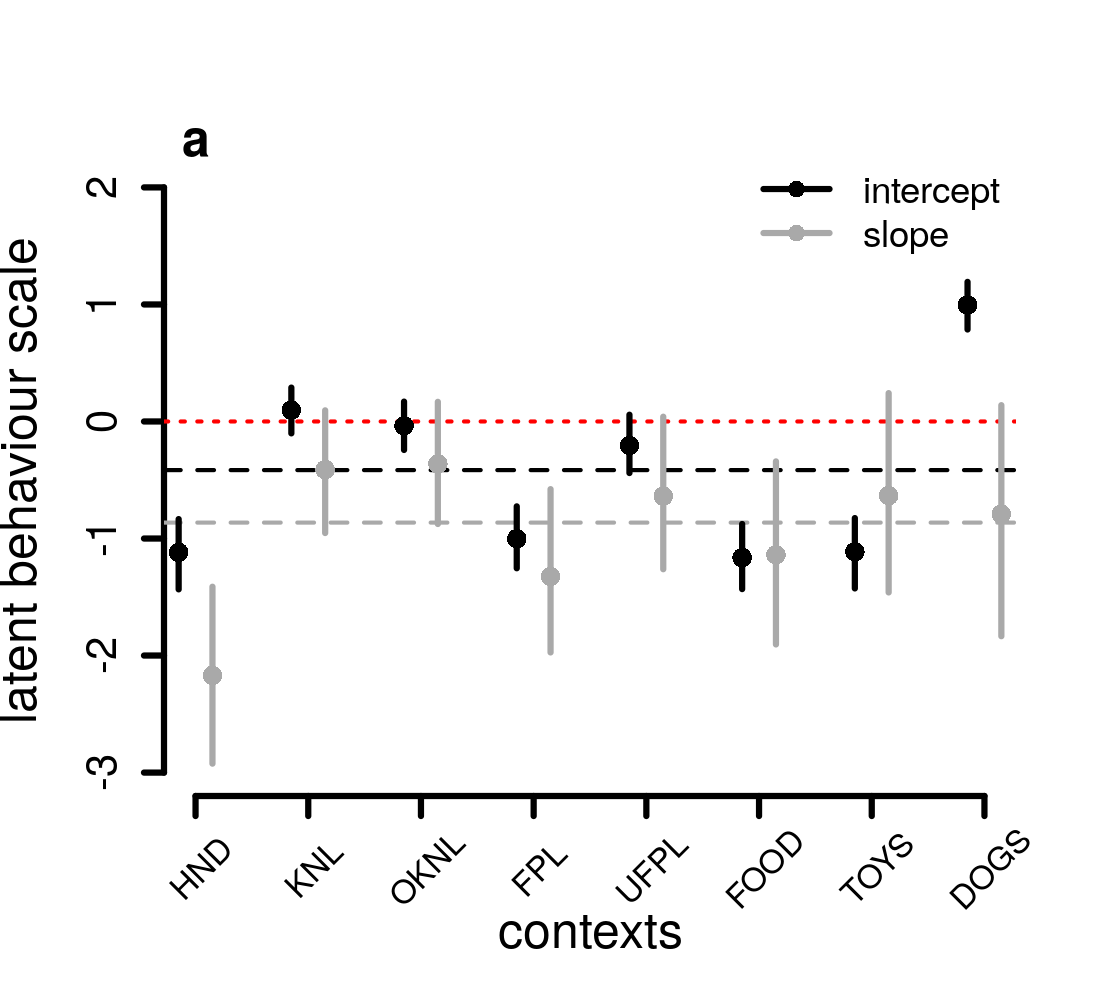
\includegraphics[scale=0.6]{figures/figure_S1_a}
  \end{subfigure}%
  ~
  \begin{subfigure}{0.5\textwidth}
    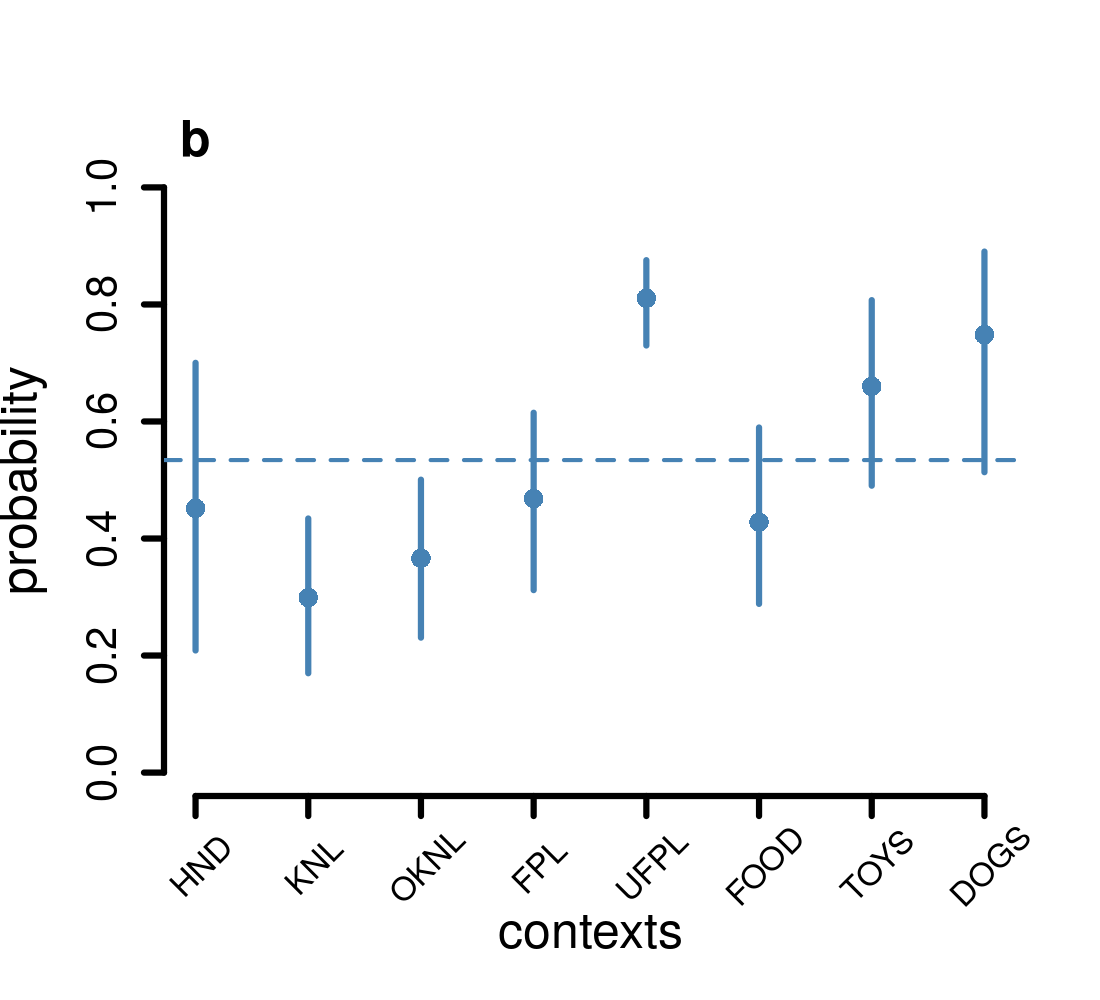
\includegraphics[scale=0.6]{figures/figure_S1_b}
  \end{subfigure}%
\caption{Variation across contexts at the shelter for latent behavioural scores (panel a; higher intercept scores indicate higher changes of amber and red codes, more positive slopes indicate higher chances of amber and red codes through time) and the probability of missing data (panel b). The red dotted line in panel a highlights zero, while the dashed coloured lines in both panels indicate the average values across contexts.
}
\label{fig_1}
\end{figure}

\begin{figure}[]
  \centering
  \begin{subfigure}{0.5\textwidth}
    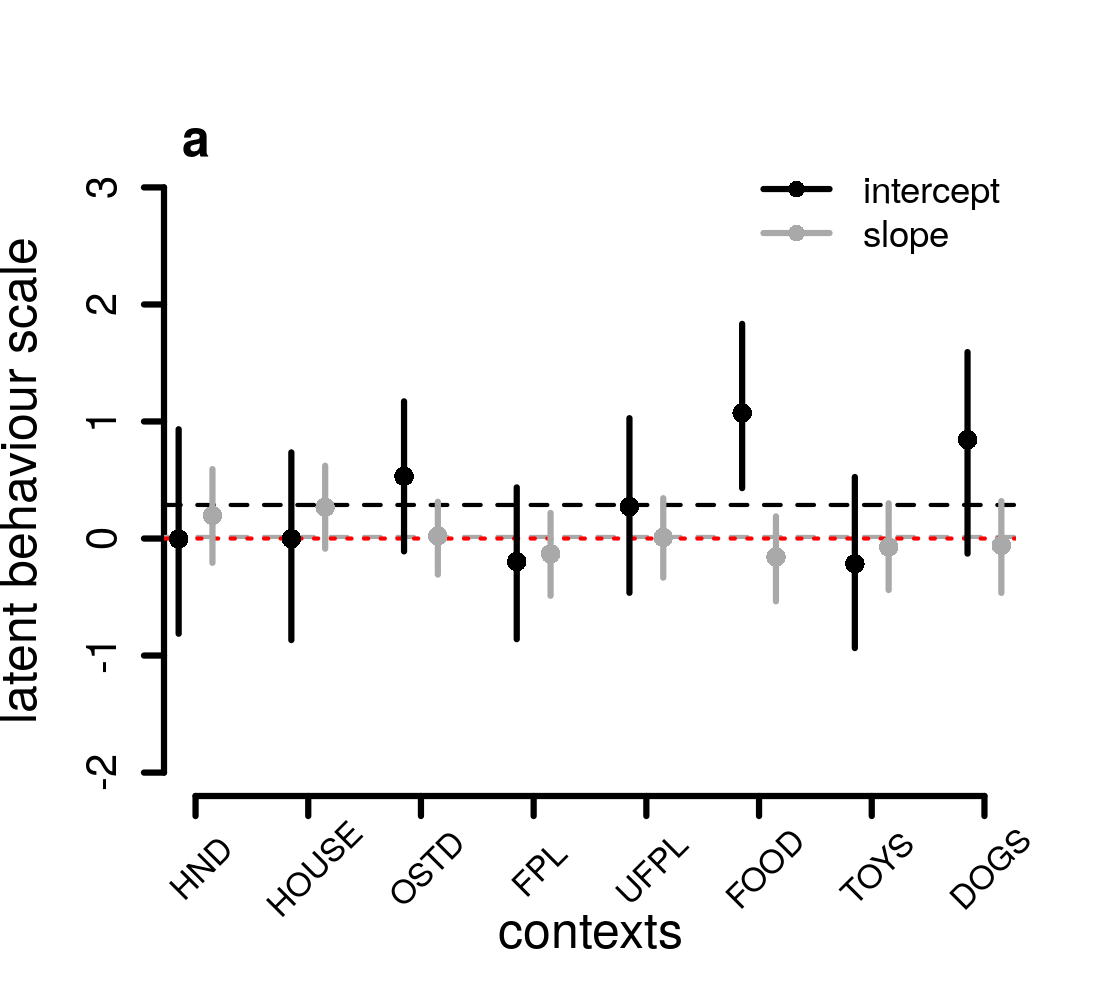
\includegraphics[scale=0.6]{figures/figure_S2_a}
  \end{subfigure}%
  ~
  \begin{subfigure}{0.5\textwidth}
    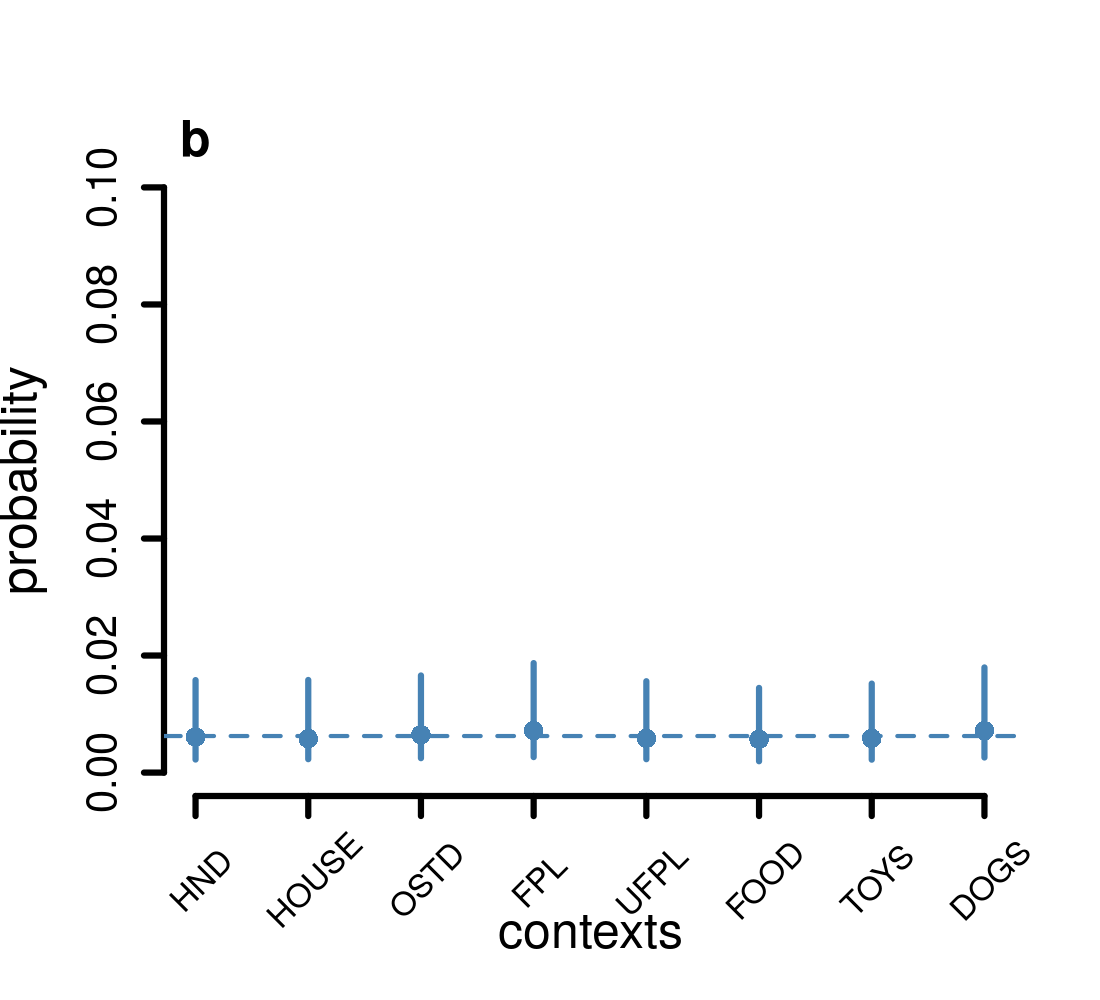
\includegraphics[scale=0.6]{figures/figure_S2_b}
  \end{subfigure}%
\caption{Variation across contexts post-adoption for latent behavioural scores (panel a; higher intercept scores indicate higher changes of amber and red codes, more positive slopes indicate higher chances of amber and red codes through time) and the probability of missing data (panel b). The red dotted line in panel a highlights zero, while the dashed coloured lines in both panels indicate the average values across contexts.
}
\label{fig_2}
\end{figure}

\newpage
\section{Repeatability}
Repeatability is the proportion of behavioural variance attributable to between-individual differences. The model used here had four sources of behavioural variance (i.e. not including the missing data component) for both the shelter ($s$) and post adoption ($a$) sub-models: variation across dogs ($\sigma_{j}^{s,a}$), variation across contexts ($\sigma_{g}^{s,a}$), variation across dog $\times$ context combinations ($\sigma_{j \times g}^{s,a}$), and error variance ($\sigma$ or $\epsilon$, respectively). Therefore, we estimated repeatability across dogs, across contexts, and across dog $\times$ context combinations separately. For example, repeatability for dog $\times$ context combinations at the shelter was calculated as:

\begin{equation}
  R_{j \times g}^{\text{shelter}} = \frac{(\sigma_{j \times g}^{s})^2}{(\sigma_{j}^{s})^2 + (\sigma_{g}^{s})^2 + (\sigma_{j \times g}^{s})^2 + \sigma^2}
\end{equation}
%
and repeatability for contexts post adoption was calculated as:

\begin{equation}
  R_{g}^{\text{adoption}} = \frac{(\sigma_{g}^{a})^2}{(\sigma_{j}^{a})^2 + (\sigma_{g}^{a})^2 + (\sigma_{j \times g}^{a})^2 + \epsilon^2}
\end{equation}

\newpage
\section{Random effect correlations}
The full list of random effect correlations estimated by the above model is presented in Table S1 found at \href{https://github.com/cmgoold/goold-newberry-lba/tree/master/paper}{https://github.com/cmgoold/goold-newberry-lba/tree/master/paper}.

\newpage
\section{Examples of individual-level posterior predictions}


\end{document}
